\documentclass[__main__.tex]{subfiles}

\begin{document}
\textbf{Э-09}\\

Закон Кулона, напряжённость поля, силовые линии электростатического поля, электростатическая защита. Работа в электростатическом поле, потенциальность электростатического поля.\\

Закон Кулона\\
Для постоянного электрического поля уравнения Максвелла имеют вид:
$$ div \vec{E} = 4 \pi \rho$$
$$ rot \vec{E} = 0$$
Абсолютная величина напряженности поля $E$ будет зависеть только от расстояния $R$ до заряда $e$. Для нахождения этой абсолютной величины применим уравнение $$ div \vec{E} = 4 \pi \rho$$ в интегральной форме $$\oint \vec{E} df = 4 \pi \int \rho dV$$.\\
Поток электрического поля через шаровую поверхность с радиусом $R$, проведенную вокруг заряда $e$, равен $4\pi R^2 E$; этот поток должен быть равен $4\pi e$. Тогда:\\
$$E = \frac{e}{R^2}$$
В векторном виде:
$$\vec{E} = \frac{e \vec{R}}{R^3}$$
Это и есть закон Кулона(Поле, создаваемое точечным зарядом, обратно пропорционально квадрату расстояния до этого заряда)
Напряженность поля.\\
$\vec{A}$ -- векторный потенциал поля.\\
Силу первого рода, отнесенную к заряду, равному единице, называют напряженностью электрического поля:\\
$$\vec{E} = -\frac{1}{c}\frac{\partial \vec{A}}{\partial t}-grad \phi$$
Для того чтобы описать электрическое поле, нужно задать вектор напряженности в каждой точке поля. Это можно сделать аналитически или графически. Для этого пользуются силовыми линиями – это линии, касательная к которым в любой точке поля совпадает с направлением вектора напряженности $\vec{E}$:\\
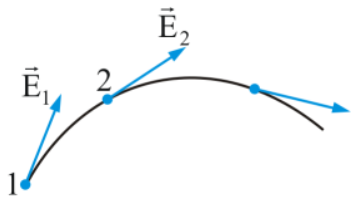
\includegraphics[width=.5\linewidth]{img/e-09-1}\\
Для системы зарядов, как видим, силовые линии направлены от положительного заряда к отрицательному:\\
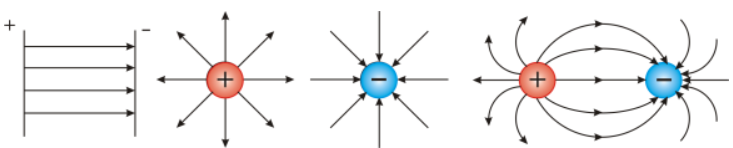
\includegraphics[width=.9\linewidth]{img/e-09-2}\\
Электростатическая защита.\\
Электростатическая защита – защита приборов и оборудования, основанная на том, что напряженность электростатического поля внутри проводника равна нулю.\\
Потенциал электростатического поля:
$$\phi = \frac{e}{R}$$
Работа поля по перемещению заряда из одной точки в другую, называется разностью потенциалов.\\
\end{document}